% The Catholic University of America PhD Dissertation Template (2021/03/23)

% This is a dissertation template for The Catholic University of America based of the Turabian Formatting for Theses and Dissertations.

% * CUA's Dissertation handbook can be found at https://graduate-studies.catholic.edu/doctoral/handbook.html

% * Developed using the turabian-formatting package (2018/08/01), available through CTAN: http://www.ctan.org/pkg/turabian-formatting

% ## Additional document class formatting options:

% natbib commands was used for the bibliography and references. 
% * Citation commands can be found at https://www.overleaf.com/learn/latex/natbib_citation_styles

% Solar Physics Journal bibligraphy format was used 
% * For instructions of bibliography access https://www.springer.com/journal/11207/submission-guidelines#Instructions%20for%20Authors_Additional%20Instructions

% ## Additional commands
% * raggedright: ragged right formatting without hyphenations
% * authordate: support for the author-date citation style
% * endnotes: support for endnotes

% This template can also be found at GitHub page at https://github.com/luiz0992/thesis_template_cua
% Adapted by Luiz F. G. dos Santos (2021/03/23)

\documentclass[12pt]{turabian-thesis}

\usepackage{lipsum}
\usepackage{blindtext}
\usepackage{longtable}
\usepackage{pdflscape}
\usepackage{graphicx}
\usepackage{verbatim}
\usepackage{color}
\usepackage{booktabs}
\usepackage{hyperref}
\usepackage{natbib}
\usepackage{tabularx}
\usepackage{amsmath}
\usepackage{mathtools}
\usepackage{array}
\usepackage{multirow}
\usepackage[normalem]{ulem}
\usepackage{xspace}
\usepackage{xcolor}
\usepackage[varg]{txfonts}
\usepackage{colortbl,dcolumn}
\newcommand\hmmax{0}
\newcommand\bmmax{0}
\usepackage{bm}
\usepackage{ragged2e}


\setcounter{secnumdepth}{3}
\setcounter{tocdepth}{2}

\makeatletter
    \renewcommand*{\l@section}{%
        \ifnum \c@tocdepth >\z@ \vskip \tf@singlelineskip \fi
        \@dottedtocline{1}{1.25in}{0.5in}}
    \renewcommand*{\l@subsection}{%
        \ifnum \c@tocdepth >\z@ \vskip \tf@singlelineskip \fi
        \@dottedtocline{2}{1.75in}{0.5in}}
\makeatother
% Information for title page
\title{SEARCH FOR DARK MATTER PRODUCED IN ASSOCIATION WITH MONOTOP IN THE FULLY
LEPTONIC CHANNEL IN PROTON-PROTON COLLISIONS AT 13 TEV WITH THE COMPACT
MUON SOLENOID EXPERIMENT}

%\subtitle{A Template based on Turabian's \emph{A Manual for Writers}, 9th edition}
\author{Rishabh Uniyal}

%FILL OUT YOUR CORRECT INFORMATION HERE!!!
\authorinfo{Ph.D., The Catholic University of America, 2022}
\department{Department of Physics}
\school{School of Arts and Science}
\institution{The Catholic University of America}
\location{Washington, D.C.}
\degreework{Doctor of Philosophy}

%For List of figures and table titles excluded word from capitalization 
% \Addlcwords{the of into in to a at on and is for}

% \makenomenclature

\begin{document}

% \renewcommand{\thepage}{\roman{page}}

\frontmatter
\maketitle
\begin{center}
    \MyTitle \\
    \vspace*{0.5\baselineskip}
    \MyAuthor~[TITLE CONFERRED UPON GRADUATION] \\
    \vspace*{0.5\baselineskip}
    Director: [Aaron Dominguez] [Professor]
\end{center}
\thispagestyle{empty}

\begingroup
\renewcommand{\clearpage}{}
\singlespacing


% \chapter*{ABSTRACT}
\vspace*{\stretch{1}} 

abstracts
\noindent
% INDEX WORDS: Georgia Southern, Thesis, ETD, Lorem ipsum.
\vspace*{\stretch{4}}
\thispagestyle{empty}

\endgroup



\PrintCommitteeInfoPage{[AUTHOR'S NAME]}{Dr. Aaron Dominguez}{Dr. Rachel Bartek}{Dr. Grzegorz Kalicy}

\chapter{DEDICATION}
\begin{center}
	\vspace*{\stretch{1}}
	
	[Optional Text]
	
	\vspace*{\stretch{4}}
\end{center}

\begin{center}
	\vspace*{\stretch{1}}
	
	\begin{FlushLeft}
	\textit{``Dedicated to my entire Uniyal clan”}\\
	\end{FlushLeft}
	\begin{FlushRight}
    [Author of the citation]
	\end{FlushRight}

	\begin{FlushLeft}
	\textit{``A inspirational citation"}
	\end{FlushLeft}
	\begin{FlushRight}
    [Author of the inspirational citation]
	\end{FlushRight}

	
	\vspace*{\stretch{4}}
\end{center}

\chapter{ACKNOWLEDGEMENTS}
\vspace{\baselineskip}
\doublespacing


I would like to thank a lot of people in this journey, I would like to start by thanking myself for being brave, for taking risks, for motivating myself to keep fighting and finishing this dissertation
\tableofcontents 
\listoffigures
\listoftables
\mainmatter

\chapter{Introduction}
\label{chapter:introduction}

%\section{An Interesting Section}
%\label{section:interesting_section}

The Standard Model (SM) of Particle Physics is one of the most complete and versatile theories which describes the fundamental particles and the forces with which they interact. The SM has been successful at describing many features of the nature that we have observed in our experiments. From the precise measurement of the electron's magnetic dipole moment to the discovery of the Higgs Boson. The predictions of the SM have just been too good. While the SM may has been really successful, there are some phenomenon like absence of the description of Dark Matter (DM) in the SM which prevents it from taking the title of the most complete and unified theory.

Dark Matter  is a form of material that neither emits, absorbs or reflects any Electromagnetic Radiation. It does seem to have mass given its Gravitational effects. Dark Matter contributes to around 24\% of the total mass energy of the universe (or 5 times the mass of ordinary matter) but does not interact directly with light, so we have not observed it yet. Astrophysical observations like Gravitational Lensing [2] (bending of light coming from distant galaxies by massive galaxies or galaxy clusters) and motion of galaxies at speeds so high for ordinary matter to sustain, Galaxy Cluster Collisions [3] and Dark Matter seeded Galaxy formations [4] have provided evidence for the presence of Dark Matter.

There are different ways in which Dark Matter could be detected-- direct detection, indirect detection and making Dark Matter on the Earth and then detecting it. The Large Hadron Collider (LHC) collides proton beams at the highest energy in the world. The proton beams collide at four main interaction points at the LHC. At each interaction point is a detector. In this thesis we will show the search for Dark Matter, based on the proton-proton collision data recorded by the Compact Muon Solenoid (CMS) experiment at the LHC.



\begin{quotation}
    \noindent Here is a block quotation---a passage from a text you found insightful and wanted to share with others. Maybe it is from a journal article, website, or book. Irrespective, it should support the argument being made.\footnote{A citation for the quoted material.}
\end{quotation}

%Maybe a sentence or two that bring the argument and evidence together.\citep{dos_santos_2020}

Check appendix \ref{appendix: chapter1}

\begin{figure} [ht]
\centering
         
\includegraphics[width=0.9\textwidth,clip=]{Figures/Introduction/CUA_logo.png}
         \caption{CUA Logo}
         \label{CUA-logo-1}
\end{figure}


\section{Another Insightful Section}
\label{section:another_interesting_section}

More ideas that really make this a great paper. Maybe a footnote or two.\footnote{Some peripheral thoughts that belong in a note.}

\chapter{Theoretical Motivations for Dark Matter Search}
\label{chapter:two}
\section{An Interesting Section}

Great thoughts that further your argument. This includes lots of strong evidence presented throughout several paragraphs, each accompanied by necessary citations.
\begin{quotation}
    \noindent Here is a block quotation---a passage from a text you found insightful and wanted to share with others. Maybe it is from a journal article, website, or book. Irrespective, it should support the argument being made.\footnote{A citation for the quoted material.}
\end{quotation}

Check appendix \ref{appendix: chapter2}
%Maybe a sentence or two that bring the argument and evidence together.\citep{dos_santos_2020}

\begin{table}[h!]
  \centering
  \caption{Very imporant table.}
  \label{tab:average_channels}
  \begin{tabular}{cc}
    \toprule
     AIA channel (\AA) &  Scaling unit [DN/s/pixel] \\
     \midrule
      94 &   10  \\
      131 &   80  \\
      171 & 2000  \\
      193 & 3000  \\
      211 & 1000  \\
      304 &  500  \\
      335 &   80  \\
      \bottomrule
  \end{tabular}
\end{table}


\section{Another Insightful Section}

More ideas that really make this a great paper. Maybe a footnote or two.\footnote{Some peripheral thoughts that belong in a note.}

\chapter{The CMS Experiment at the LHC}
\label{chapter:three}
\section{The Large Hadron Collider}

The Large Hadron Collider (LHC) is the world’s largest and most powerful particle accelerator. Inside the accelerator, two highly energetic proton beams collide up to a center-of-mass energy of 14 TeV. The LHC is constructed inside a 27 km tunnel, 100 m under the ground, located partly in Switzerland and France.

At the LHC two energetic proton beams travel in opposite directions in separate beam pipes. The proton beams travel in bunches separated by 25 ns in time. The beams travel at relativistic speeds and collide at four major interaction points at the LHC. The LHC has four main detector experiments at each interaction point: ALICE (A Large Ion Collider Experiment), ATLAS (A Toroidal LHC Apparatus), CMS (Compact Muon Solenoid), and LHCb (Large Hadron Collider beauty). ATLAS and CMS are general purpose-detectors with broad physics objectives ranging from studying the Standard Model to searching Beyond Standard Model (BSM) physics such as Dark Matter. While ALICE and LHCb are more physics dedicated detectors, ALICE and LHCb are dedicated to heavy-ion physics and studying b-quark physics respectively.

%\begin{quotation}
%    \noindent Here is a block quotation---a passage from a text you found insightful and wanted to share with others. Maybe it is from a %journal article, website, or book. Irrespective, it should support the argument being made.\footnote{A citation for the quoted material.}
%\end{quotation}

%Check appendix \ref{appendix: chapter3}

%Maybe a sentence or two that bring the argument and evidence together.\citep{dos_santos_2020}



\section{The Compact Muon Solenoid Experiment}
\subsection{Introduction}
The Compact Muon Solenoid (CMS) is a general purpose detector located in eastern France at the Large Hadron Collider (LHC) tunnel 100 m underground. It is a general purpose detector because of its broad physics searches ranging from studying the Standard Model (SM) to searching for particles that could potentially make Dark Matter (DM). CMS is a cylindrical shaped detector with 21 m in length and 15 m in cross-sectional diameter. The three main characteristics of the CMS experiment are its compactness, accurate detection of Muon particles in the muon system and its magnetic solenoid. The superconducting magnetic solenoid at the core of the CMS detector produces a continuous magnetic field of 3.8 T which is of the order of O(5) of Earth's magnetic field (0.25 - 0.65 gaus). Such large magnetic field is required for a precise measurement of the momentum of high-energy charged particles. All CMS detector subsystems are enclosed by the magnetic solenoid, the muon system, on the other hand, is on the outside. Muons are the particles that are directly detected by the CMS, with a special property that they neither stop nor decay within the boundaries of the detector. They undergo very little energy loss and thus act as a powerful medium to study high-energy process in the presence of high background.
The CMS detector is cylindrical shaped with an onion like structure, having several concentric layers of subsystems. These subsystems help prepare "photographic images" of each collision event by determining the properties of the particles in the collision. CMS has the following basic subsystems ordered from innermost to outermost:

\begin{enumerate}
    \item Silicon Tracker
    \item Electromagnetic Calorimeter
    \item Hadronic Calorimeter
    \item Superconducting Solenoid Magnet
    \item Muon System
    
    
\end{enumerate}
The CMS detector can detect 5 general categories of particles as shown in the figure below:
 \begin{enumerate}
    \item Electrons
    \item Photons
    \item Charged Hadrons
    \item Neutral Hadrons
    \item Muons
\end{enumerate}

\begin{figure} [ht]
\centering
         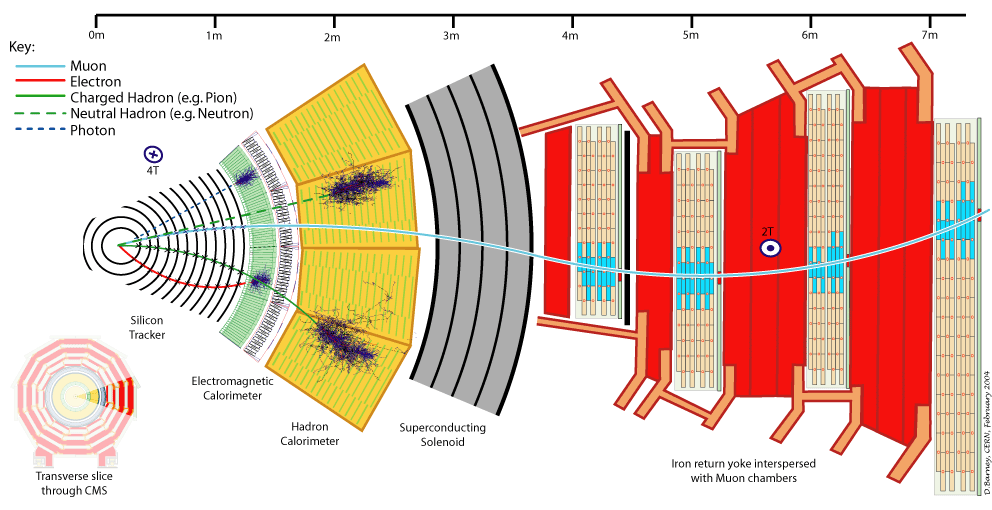
\includegraphics[width=0.9\textwidth,clip=]{thesis_template_cua/Figures/CMS_LHC_chapter/CMSSlice.png}
         \caption[#CMS Slice]{This Figure shows the cross-sectional slice of the CMS detector. Here we have shown the different sub-systems of CMS, trajectories and energy deposits of the 5 general categories of particles detected by CMS by one or more of its sub-systems}
         \label{cms_slice}
\end{figure}
%More ideas that really make this a great paper. Maybe a footnote or two.\footnote{Some peripheral thoughts that belong in a note.}
\subsection{Coordinate System}


\subsection{Silicon Tracker}

\subsection{Electromagnetic Calorimeter}

\subsection{Hadronic Calorimeter}

\subsection{Solenoid Magnet}

\subsection{Muon System}

\subsubsection{DT}

\subsubsection{RPC}

\subsubsection{CSC}

\subsection{Trigger System}
\chapter{Theoretical Foundations of Monotop Analysis}
\label{chapter:four}
This Chapter will focus on the explaining the theory behind the monotop analysis and the importance of the top quark.
\section{Monotop Analysis}

Great thoughts that further your argument. This includes lots of strong evidence presented throughout several paragraphs, each accompanied by necessary citations.
\begin{quotation}
    \noindent Here is a block quotation---a passage from a text you found insightful and wanted to share with others. Maybe it is from a journal article, website, or book. Irrespective, it should support the argument being made.\footnote{A citation for the quoted material.}
\end{quotation}
%Maybe a sentence or two that bring the argument and evidence together.\citep{dos_santos_2020}



\section{The Top quark}

The top quark was discovered the Fermilab Tevatron almost 25 years ago. It is the weak isospin partner of the bottom quark. Its discovery resulted in completion of the three generation structure of the standard model (SM). The top quark mass was measured to be $m_{t} = 176 \pm 13$ GeV, a charge of 2/3 times the charge on the electron and a lifetime of $5 \times 10^{-25} s$ making it the heaviest of all the fermions known till date in the standard model. Because of it's large mass and correspondingly short lifetime it behaves differently than other quarks. 

The top quark decays before it hadronizes, passing its information to the decay products. Therefore making it possible to infer its properties from the decay products in the detector. The top quark decays into a a bottom quark and a W boson, and since the W boson is an unstable particle it decays into a quark anti-quark pair of different flavors (hadronic decay channel) or to a charged lepton and a neutrino (leptonic decay channel) with the following branching ratios.

\begin{table}[h!]
  \centering
  \caption{}
  \label{tab:average_channels}
  \begin{tabular}{cc}
    \toprule
     Decay channel &  Branching ratio \\
     \midrule
      $W^{\pm} \rightarrow q\Bar{q'}$ &   $68.32\%$  \\
      $W^{\pm} \rightarrow e^{\pm} \Bar{\nu_{e}}$ &   $10.46\%$  \\
      $W^{\pm} \rightarrow \mu^{\pm} \Bar{\nu_{\mu}}$ &   $10.50\%$  \\
      $W^{\pm} \rightarrow \tau^{\pm} \Bar{\nu_{\tau}}$ &   $10.75\%$  \\
      \bottomrule
  \end{tabular}
\end{table}

As the top quark decays into a W boson and a bottom quark, it's evident that the hadronic and leptonic decay probabilities of the top quark will be proportional to the hadronic and leptonic decay probabilities of the W boson. So, it can be implied from the above table that, around 70\% of times the top quark decays into three quarks (two quarks from W boson and one bottom quark) which further hadronize to produce jets. While around 30\% of the times the top quark would decay leptonically to a lepton, its corresponding lepton neutrino and a bottom quark. In this thesis we will be exploring the leptonic channel for the search for Dark Matter (DM), so our final state signature would a lepton, its corresponding neutrino and a jet coming from a bottom quark.

In accordance with the SM, at the LHC, top quarks are predominantly produced in pairs ($t \Bar{t}$) through strong interactions and as single top via the electroweak interaction. In the following section we will be looking at the production of a single top quark (Monotop) in association with missing transverse energy due to the two DM candidates, as an extension to the SM. 


\section{The Monotop Model}
\chapter{Conclusion}
\label{chapter:conclusion}


\section{An Interesting Section}

Great thoughts that further your argument. This includes lots of strong evidence presented throughout several paragraphs, each accompanied by necessary citations.
\begin{quotation}
    \noindent Here is a block quotation---a passage from a text you found insightful and wanted to share with others. Maybe it is from a journal article, website, or book. Irrespective, it should support the argument being made.\footnote{A citation for the quoted material.}
\end{quotation}
Maybe a sentence or two that bring the argument and evidence together.\citep{dos_santos_2020}



\section{Another Insightful Section}

More ideas that really make this a great paper. Maybe a footnote or two.\footnote{Some peripheral thoughts that belong in a note.}



\backmatter

\bibliographystyle{unsrt}
\bibliography{backmatter/refferences}

    \begin{appendixes}
    \chapter{Chapter 1}\label{appendix: chapter1}

\begin{figure}
\centering
         
\includegraphics[width=0.5\textwidth,clip=]{Figures/Introduction/CUA_logo_2.png}
         \caption{CUA Logo 2}
         \label{CUA-logo-2}
\end{figure}
    \end{appendixes}

    \begin{appendixes}
    \chapter{Chapter 2}\label{appendix: chapter2}

\lipsum[4-5]
    \end{appendixes}
    
    \begin{appendixes}
    \chapter{Chapter 3}\label{appendix: chapter3}

\lipsum[4-5]
    \end{appendixes}
    

\end{document}
